% Chapter X

\chapter{Protoloco P2P} % Chapter title

\label{ch:protocolo_p2p} % For referencing the chapter elsewhere, use \autoref{ch:name} 

Una red peer-to-peer (P2P) o red de pares, es una red de computadoras en la que todos o algunos aspectos de ésta, funcionan sin clientes ni servidores fijos, sino una serie de nodos que se comportan como iguales entre sí. Es decir, actúan simultáneamente como clientes y servidores respecto a los demás nodos de la red \cite{wiki_p2p}.

Las redes peer-to-peer aprovechan, administran y optimizan el uso del ancho de banda de los demás usuarios de la red por medio de la conectividad entre los mismos, obteniendo más rendimiento en las conexiones y transferencias que con algunos métodos centralizados convencionales, donde una cantidad relativamente pequeña de servidores provee el total del ancho de banda y recursos compartidos para un servicio o aplicación.
Alfredo F. nos dice que de forma simple puede verse como la comunicación entre pares o iguales utilizando un sistema de intercambio \cite{bordignon:2005}.

Los sistemas compañero a compañero (o P2P por sus siglas en inglés) permiten que computadoras de usuario final se conecten directamente para formar comunidades, cuya finalidad sea el compartir recursos y servicios computacionales. En este modelo, se toma ventaja de recursos existentes en los extremos de la red, tales como tiempo de CPU y espacio de almacenamiento. Las primeras aplicaciones  emergentes se orientaban a compartir archivos y a la mensajería \cite{bordignon:2005}.


%----------------------------------------------------------------------------------------

\section{Clasificación}

\subsection{Directorio Centralizado}

Esta primera visión se puso en práctica para el año 1997 con la red Napster \cite{rfc4981}. Bajo este modelo los clientes o peers realizan el descubrimiento y búsqueda de los otros miembros mediante un servidor central, luego el mismo servidor se encarga de negociar la conexión entre ambos clientes.

Este tipo de red P2P se basa en una arquitectura monolítica en la que todas las transacciones se hacen a través de un único servidor que sirve de punto de enlace entre dos nodos y que, a la vez, almacena y distribuye los nodos donde se almacenan los contenidos. Poseen una administración muy dinámica y una disposición más permanente de contenido. Sin embargo, está muy limitada en la privacidad de los usuarios y en la falta de escalabilidad de un sólo servidor, además de ofrecer problemas en puntos únicos de fallo, situaciones legales y enormes costos en el mantenimiento así como el consumo de ancho de banda \cite{wiki_p2p}.

El principal problema presentado en este modelo es que el servidor P2P Central es un posible punto de quiebre que pueda atentar contra la estabilidad de la red.

\begin{figure}[h]
  \centering
    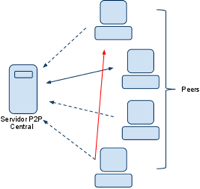
\includegraphics[scale=1]{gfx/p2p_central}
  \caption{Directorio Centralizado}
  \label{conexionhttp}
\end{figure}

%------------------------------------------------

\subsection{Directorio Distribuido}

Uno de los ejemplos más conocidos de este tipo de redes es Freenet \cite{rfc4981}. Las redes P2P de este tipo son las más comunes, siendo las más versátiles al no requerir de un gestionamiento central de ningún tipo, lo que permite una reducción de la necesidad de usar un servidor central, por lo que se opta por los mismos usuarios como nodos de esas conexiones y también como almacenistas de esa información. En otras palabras, todas las comunicaciones son directamente de usuario a usuario con ayuda de un nodo (que es otro usuario) quien permite enlazar esas comunicaciones \cite{wiki_p2p}.

\begin{figure}[h]
  \centering
    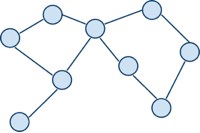
\includegraphics[scale=1]{gfx/p2p_distribuido}
  \caption{Solución Distribuida}
  \label{conexionhttp}
\end{figure}

%------------------------------------------------

\subsection{Directorio Híbrido}

Un ejemplo de este tipo de redes es Gnutella 0.6 \cite{sanghi}. Este tipo de red se encuentra formada por una estructura jerárquica la cual comprende nodos de usuario y ultrapeers. Cuando un nuevo nodo entra al sistema, este se transforma como un nodo usuario quedando en el perímetro de la red, donde éste no posea ninguna responsabilidad de enrutamiento y su única función es la de enviar consultas a los ultrapeers. 

Por otro lado nodos con capacidades más elevadas y con habilidades de procesamiento mejoradas, son promovidos como ultrapeers. Éstos son los responsables de realizar enrutamiento y de resolver consultas de los nodos usuario \cite{sanghi}. 

\begin{figure}[h]
  \centering
    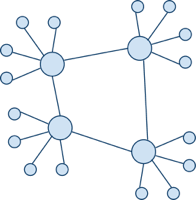
\includegraphics[scale=1]{gfx/p2p_dir_centralizado}
  \caption{Directorio Híbrido}
  \label{conexionhttp}
\end{figure}

%----------------------------------------------------------------------------------------

\section{Mecanismos de búsqueda en Redes P2P}
Las redes P2P son clasificadas a su vez en: Redes no estructuradas y Redes estructuradas. Algunos han aseverado que éstos algoritmos son alternativas que compiten entre sí \cite{rfc4981}.

\begin{description}

\item[Redes No Estructuradas: ]
Las redes No Estructuradas han sido llamadas redes de "primera generación". Los nodos en estas redes se unen conectándose a través de cualquier otro nodo. En los primeras versiones de Gnutella, ésta se podía clasificar como No Estructurada \cite{rfc4981}. En estas redes el costo por enrutamiento debido difusión o broadcasting es muy elevado o también puede ocasionar que hayan fallos encontrando el recurso solicitado. \cite{rfc4981}

\item[Redes Estructuradas: ]
Las redes estructuradas tienen importantes ventajas. Proporcionan un mecanismo determinista de localización, de tal forma que se asegura que un recurso será encontrado siempre que esté en la red. Además, los mensajes de búsqueda son encaminados de forma eficiente, de tal forma que el recurso es encontrado en $O(\log n)$ saltos, donde $n$ es el tamaño de la red \cite{wiki_p2p}. Estas redes han sufrido dos críticas principalmente \cite{rfc4981}. La primera de ellas es entorno a la transitoriedad de un nodo, que al final afecta qué tan robusto es la red. La otra crítica es debido a que éstas redes no soportan búsquedas por palabra clave ni consultas complejas como los sistemas No Estructurados. 

\end{description}